%%\documentclass[10pt, twocolumn]{article}
\documentclass{article}
\usepackage[margin=1in]{geometry}
\usepackage{graphicx}
\usepackage{cite}
\usepackage{algpseudocode}
\usepackage{listings}

\title{Hulaan Mo: Some Notes on Cryptography}
\author{Shiela Kathleen L. Borja\\Joseph Anthony C. Hermocilla\\Mark Froilan B. Tandoc}
\date{}


\begin{document}
\maketitle

\section{Introduction}
Cryptography is an area of study of encryption of plaintext to a so called ciphertext. Cryptographic systems are characterized along three independent dimensions. First is the type of operations used for transforming plaintext to ciphertext. All encryption algorithms are based on two general principles: \textit{substitution} where each element in the plaintext is mapped into another element, and \textit{transposition} where elements in the plaintext are rearranged. Second is the number of keys used. If both sender and receiver use the same key, the system is referred to as \textit{symmetric}, single-key, secret-key, or conventional encryption. If the sender and receiver use different keys, the system is referred to as \textit{asymmetric}, two-key, or public-key encryption. Last dimension is the way in which the plaintext is processed. A \textit{block cipher} processes the input one block of elements at a time, producing an output block for each input block. A \textit{stream cipher} processes the input elements continuously, producing output one element at a time \cite{stallings2011}.

There are two types of attack on an encryption algorithm. \textit{Cryptanalysis} is based on properties of the encryption algorithm and \textit{brute-force} which involves trying all possible keys.

\section{Classical Encryption Techniques}
\subsection{Caesar Cipher}
The earliest and simplest known substitution cipher by Julius Caesar \cite{stallings2011}. This cipher involves replacing each letter of the alphabet with the letter standing three places (or even more for the general algorithm) further down the alphabet. The alphabet is wrapped around where Z follows A. For example:
\\

\begin{tabular}{r l}
	plain: & COMSCI IS THE BEST\\
	cipher: & FRPVFL LV WKH EHVW
\end{tabular}
\\

If the attacker knew that Caesar cipher was used, brute-force cryptanalysis is easily performed and there are only 25 keys to try.

\subsection{Monoalphabetic Cipher}
It was shown that Caesar cipher is far from secure. The key space can be dramatically increased if we allow arbitrary substitution for each letter/character. With this, the number of possible keys is increased from 25 to the number of permutations for the given alphabet or 26! possible keys. There is still, however, another possible attack. If the cryptanalyst knew the nature of the plaintext (e.g. noncompressed English text), then he/she can exploit the regularities of the language like relative frequency of the letters in the ciphertext and compare it to the standard frequency distribution for English \cite{stallings2011}.

\subsection{Playfair Cipher}
The Playfair algorithm uses a 5 x 5 matrix of letters constructed using a keyword. The matrix is constructed by filling in the letters of the keyword (minus duplicates) from left to right and from top to bottom. Then filling the remainder of the matrix with the remaining letters in alphabetical order. The letters I and J count as one letter \cite{stallings2011}. For example with keyword \textit{monarchy}:
\\

\begin{tabular}{|c|c|c|c|c|}
\hline
M & O & N & A & R\\
\hline
C & H & Y & B & D\\
\hline
E & F & G & I/J & K\\
\hline
L & P & Q & S & T\\
\hline
U & V & W & X & Z\\
\hline
\end{tabular}
\\

The plaintext is encrypted two letters at a time, according the the rules:
\begin{itemize}
\item Repeating plaintext letters that are in the same pair are separated with a filler letter, such as x, so that balloon would be treated as ba lx lo on.
\item Two plaintext letters that fall in the same row of the matrix are each replaced by the letter to the right, withe first element of the row circularly following the last. For example, ar is encrypted as RM.
\item Two plaintext letters that fall in the same column are each replaced by the letter beneath, with the top element of the column circularly following the last. For example, mu is encrypted as CM.
\item Otherwise, each plaintext letter in a pair is replaced by the letter that lies in its own row and the column occupied by the other plaintext letter. Thus, hs becomes BP and ea becomes IM/JM.
\end{itemize}

The Playfair cipher is a great advancement over monoalphabetic ciphers. However, despite this level of confidence in its security, it is still relatively easy to break because it still leaves much structure of the plaintext language intact.

\subsection{Polyalphabetic Cipher}
Another way to improve monoalphabetic technique is to use different monoalphabetic substitutions through encryption of the plaintext message. The general name of the technique is polyalphabetic substitution cipher \cite{stallings2011}.

The best known and one of the simplest is the \textbf{Vigen\`{e}re cipher}. It is essentially multiple caesar ciphers. For every letter in the plaintext, we use one letter at a time of the secret key as the key to apply for the Caesar cipher. For example:
\\

\begin{tabular}{l l}
key: & deceptivedeceptive\\
plaintext: & wearediscoveredsav\\
ciphertext: & ZICVTWQNGRZGVTWAVZ\\
\end{tabular}
\\

When expressed numerically,
\\
\begin{tabular}{| l *{9}{|c} |}
\hline
key & 3 & 4 & 2 & 4 & 15 & 19 & 8 & 21 & 4\\
\hline
plain & 22 & 4 & 0 & 17 & 4 & 3 & 8 & 18 & 2\\
\hline
cipher & 25 & 8 & 2 & 21 & 19 & 22 & 16 & 13 & 6\\
\hline
\hline
key & 3 & 4 & 2 & 4 & 15 & 19 & 8 & 21 & 4\\
\hline
plain & 14 & 21 & 4 & 17 & 4 & 3 & 18 & 0 & 21\\
\hline
cipher & 17 & 25 & 6 & 21 & 19 & 22 & 0 & 21 & 25\\
\hline
\end{tabular}
\\

The length of the key can be derived by observing for repeating sequences in the cipher text. In the example, the sequence VTW occurred twice and it can be used to determine the length of the key which is 9.

To defend on such cryptanalysis, we can choose to have a very long keyword as long as the plaintext and has no statistical relationship to it. It was introduced by an AT\&T engineer Gilbert Vernam in 1918 called \textbf{Vernam Cipher} \cite{stallings2011}.

\subsection{One-Time Pad}
An Army Signal Corp officer named Joseph Mauborgne, improved the Vernam cipher that is said to be unbreakable. The key should be random and as long as the plaintext such that the key is not repeated. Moreover, new messages requires new keys of the same length as the new message. This produces random output with no statistical relationship with the plaintext, therefore no way of breaking the code. However, there are practical difficulties. One is the problem of making large quantities of random keys. Another is the problem of key distribution and protection.

\subsection{Transposition Techniques}
The techniques discussed were all substitution of a ciphertext symbol for a plaintext symbol. A different kind of mapping is by performing some sort of permutation on the plaintext letters. This is referred to as a transposition cipher \cite{stallings2011}.

The simplest of a transposition cipher is the \textbf{rail fence} technique where the plaintext is written down as a sequence of diagonals and then read off as a sequence of rows. For example, the message "\textit{meet me after the toga party}" with a rail fence of depth 2:
\\
\begin{verbatim}
m e m a t r h t g p r y
 e t e f e t e o a a t
\end{verbatim}
will yield the encrypted message:\\
MEMATRHTGPRYETEFETEOAAT

A more complex scheme is to write the message in a matrix and read the message off, column by column, but permute the order of the columns. The order of the columns would then become the key of the algorithm. For example:
\\

\begin{tabular}{l | *{7}{c}}
Key: & 4 & 3 & 1 & 2 & 5 & 6 & 7\\
\hline
Plaintext: & a & t & t & a & c & k & p\\
& o & s & t & p & o & n & e\\
& d & u & n & t & i & l & t\\
& w & o & a & m & x & y & z\\
\end{tabular}
\\

Ciphertext:\\
TTNAAPTMTSUOAODWCOIXKNLYPETZ
\\

The transposition stage can be done repeatedly to have more complex permutation to improve security.

\section{Directions of Cryptography}
\subsection{Symmetric Ciphers}
Symmetric encryption is  where encryption and decryption are performed using the same key. It is also known as conventional encryption \cite{stallings2011}. A symmetric encryption scheme has five parts:

\begin{enumerate}
	\item \textbf{Plaintext:} The original intelligible message or data.
	\item \textbf{Encryption Algorithm:} Performs various substitutions and transformations on the plaintext.
	\item \textbf{Secret Key:} It is also an input for the encryption algorithm. The exact substitutions and transformations performed by the algorithm depend on the key.
	\item \textbf{Ciphertext:} The scrambled message produced as output.
	\item \textbf{Decryption algorithm:} Essentially the encryption algorithm performed in reverse. It takes the ciphertext and the secret key as input and produces the plaintext as output.
\end{enumerate}

Other terms that are used in the sections are:
\begin{enumerate}
	\item \textbf{Field:} A set where the four fundamental operations preserving the closure property.\cite{stallings2011}
	\item \textbf{GF($2^{8}$):} defined as a finite field containing 2n elements.\cite{stallings2011}
	\item \textbf{prop ratio:} the relative amount of all input pairs that for the given input difference give rise to the output difference. \cite{daemen1999}
\end{enumerate}

\subsubsection{Block Ciphers}
Block cipher allows a block of plaintext to be treated as a whole and used to produce a ciphertext block of equal length. The simplest techniques that can be used to encrypt a block of plaintext are substitution and permutation. Substitution replaces a symbol or groups of symbols with a corresponding ciphertext symbols or groups of symbols. Permutation replaces a sequence of plaintext symbols with a permutation of the same set of symbols. \cite{stallings2011}

\subsubsection{Feistel Cipher Structure}
As discussed by Stallings \cite{stallings2011}, the inputs required in the encryption algorithm are the plaintext block of length 2w bits and a key K. The plaintext block is then divided into two halves, $L_{0}$ and $R_{0}$, which pass through n rounds of processing and then combine to create  the ciphertext. In each round, substitution is performed on the left-half block , $L_{0}$. This is done by applying a round function F to the right-half block and then applying XOR to F's output and the left-half block. The round function has the same general structure for each round but is parameterized by the round subkey $K_{i}$. The decryption algorithm for the Feistel cipher is basically the same as the encryption process with the rule: Use the ciphertext as a input to the algorithm, but use subkeys $K_{i}$  in reverse order. In order to ensure that decryption is the inverse of encryption, the final round of a Feistel cipher switches the ciphertext to ($R_{0}$, $L_{0}$). Figure \ref{FeistelEncryptDecrypt} shows the Feistel encryption and decryption processes.

\begin{figure}[h]
\begin{center}
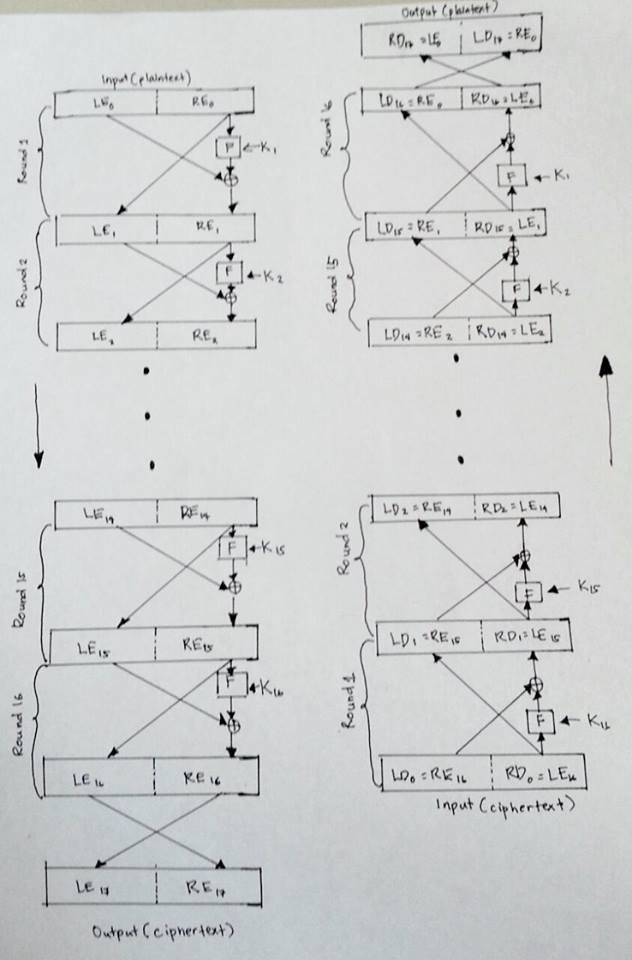
\includegraphics[scale=.2]{FeistelEncryptDecrypt2.png}
\caption{Feistel Encryption and Decryption}
\label{FeistelEncryptDecrypt}
\end{center}
\end{figure}

\subsubsection{The Data Encryption Standard (DES)}
The Data Encryption Standard is a block cipher encrypts the data in 64b blocks through a 56b key. It is the most widely used public cryptosystem in the world. It is mainly used for electronic funds transfer, civilian satellite communications security, and UNIX password protection.\cite{landau2000} DES was first proposed in 1975 and was adopted by the National Bureau of Standards(NBS) in 1977. DES was approved as the Federal Information Processing Standard 46. \cite{stallings2011}
	The development of DES can be traced back to the development of LUCIFER, a Feistel block cipher that uses 64b blocks and 128b key. LUCIFER became very promising leading IBM, its developers, to launch a new marketable commercial encryption product which can be implemented on a chip. The result of the new project was a more cryptanalysis-secure version of LUCIFER that uses 56b key. In 1973, NBS accepted proposals for a national cipher standard where IBM submitted the refined version of LUCIFER which was later adopted as the Data Encryption Standard.\cite{stallings2011}
	DES came under fire even before its adaptation as a standard due to its enormous key size reduction and its classified design criteria for its internal structure, S-boxes. The critics were concerned that the new key size is vulnerable to brute-force attacks. Also, they were concerned that the classified  design criteria might hide weak points that would enable the National Security Agency(NSA) to decipher messages without the key.\cite{stallings2011} Despite the issues surrounding DES, it remained as a strong  encryption algorithm until the mid 1990s when a USD250,000 computer built by the Electronic Frontier Foundation (EFF) decoded a DES-encoded message in 56 hours. This was later improved to 22 hours using a combination of 100,000 networked PCs and the EFF machine.\cite{landau2000}

\paragraph{DES Encryption}
As discussed by Landau\cite{landau2000}, input to the algorithm are the plaintext grouped into 64b blocks and a single 56b key. First step in the encryption is to rearrange the 64b plaintext to produce a permuted input.  Throughout the whole plaintext, a single 56b key is used to determine the transformation of all the blocks. DES uses a 48b subkey for each of the sixteen identical rounds of mixing. DES begins with  an initial permutation P and ends with its inverse, $P^{-1}$. Selecting the subkeys or “key schedule” begins with splitting the 56b key into two 28b halves. Each half is rotated one or two bits (one bit in rounds 1, 2, 9 and 16; two bits otherwise) then the two halves are put back together, and then the 48 bits are chosen and put in order as follows:

\begin{tabular}{*{6}{|c}|}
\hline
14 & 17 & 11 & 24 & 1 & 5\\
\hline
3 & 28 & 15 & 6 & 21 & 10\\
\hline
23 & 19 & 12 & 4 & 26 & 8\\
\hline
16 & 7 & 27 & 20 & 13 & 2\\
\hline
41 & 52 & 31 & 37 & 47 & 55\\
\hline
30 & 40 & 51 & 45 & 33 & 48\\
\hline
44 & 49 & 39 & 56 & 34 & 53\\
\hline
46 & 42 & 50 & 36 & 29 & 32\\
\hline
\end{tabular}

DES is a standard Feistel construction:\\
$L_{i}=R_{i-1},\\
R_{i}=L-i-1 \, xor \, f(R_{i-1}, K_{i})\\
where\\
f(R_{i-1}, K_{i})=P(S(E(R_{i}-1) \, xor \, K_{i}))\\
with \, the \, operations\\
E(expansion),S(S-boxlookup),P(permutation)
$

The expansion operation E begins with bit 32 and cycles back to the beginning, using all the bits in order, repeating every fourth and fifth bits. E allows every bit of a DES ciphertext to depend on every bit of the plaintext and every bit of the key.\cite{landau2000}

After performing XOR operation on the round subkey and the expanded right half, the result is then passed through the S-boxes. Each of the S-box takes an input of six bits and has an output of four bits. Each of the output of the eight S-boxes is concatenated producing a 32b output.\cite{landau2000}

$P^{1}$, a specific 32b permutation of the S-boxes' output, completes the round function. It carries 1, ..., 32 into the following list:
\begin{tabular}{*{8}{|c}|}
\hline
16 & 7 & 20 & 21 & 29 & 12 & 28 & 17\\
\hline
1 & 15 & 23 & 26 & 5 & 18 & 31 & 10\\
\hline
2 & 8 & 24 & 14 & 32 & 27 & 3 & 9\\
\hline
19 & 13 & 30 & 6 & 22 & 11 & 4 & 25\\
\hline
\end{tabular}

P guarantees that the output from one round of DES affects the input for the multiple S-boxes in the next round. At the end of all the rounds, DES ends with a final exchange of the left and right halves (and then $P^{-1}$).\cite{landau2000} Figure \ref{DataEncryptionStandard} shows the Data Encryption Standard.
\begin{figure}[h]
\begin{center}
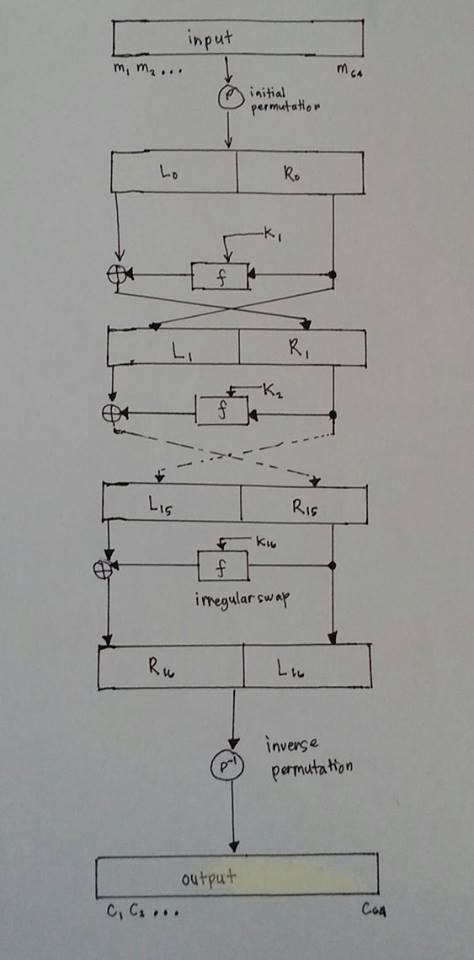
\includegraphics[scale=.4]{DataEncryptionStandard2.jpg}
\caption{The Data Encryption Standard}
\label{DataEncryptionStandard}
\end{center}
\end{figure}

\paragraph{DES Decryption}
Since DES has a Feistel cipher structure, it follows that its decryption algorithm uses the same algorithm as its encryption algorithm, except that the application of the subkey is reversed.\cite{stallings2011}

\paragraph{Attacks on DES}
It was no secret that DES was bombarded with a lot of protests regarding its small key space. A lot of its critics tried to prove that DES was not a very strong encryption algorithm. Discussed here are some of the attacks made on DES.

\subparagraph{Differential Cryptanalysis}
Pioneered by Eli Biham and Adi Shamir, differential cryptanalysis attack requires only examining $2^{47}$ texts which is lower than the $2^{56}$ required in the exhaustive search. As described by Landau\cite{landau2000}, Biham and Shamir's attack on DES is:

\begin{enumerate}
\item Pick an appropriate difference $\Delta X$.
\item Create an appropriate number of plaintext pairs with this $\Delta X$, encrypt with DES, and store the ciphertext pairs.
\item For each pair, from the plaintext $\Delta X$ and the ciphertext pair, determine the expected output difference of as many S-boxes in the last round as possible.
\item For each possible key value, count the number of pairs that result with the expected output change using the value in the last DES round.
\item The right key value is the one suggested by all the key pairs.
\end{enumerate}

\subparagraph{Linear Cryptanalysis}
The seemingly simple and unanticipated Linear Cryptanalysis attack was developed by Mitsuru Matsui. Its objective is to find an effective linear equation of the form\cite{landau2000}:\\
$P[\alpha_{1}\alpha_{2}\cdots,\alpha_{3}] \, \oplus \, C[\beta_{1}\beta_{2}\cdots,\beta_{3}] = K[\gamma_{1}\gamma_{2}\cdots,\gamma_{3}]$

Matsui determined the best linear approximate expressions for DES until 20 rounds. He then used a combination of reduced-rounds linear approximation and exhaustive search to get the key. On the average, the attack requires $2^{43}$ known plaintexts. In 1994, this attack broke a DES-encoded message in 50 days.\cite{stallings2011}

\subsubsection{Advanced Encryption Standard (AES)}
As discussed by Stallings\cite{stallings2011}, AES was first published in 2001 by the National Standards and Technology (NIST) to replace Data Encryption Standard as the approved standard for commercial purposes. The winning algorithm was first known as the Rijndael Block Cipher proposed by Joan Daemen and Vincent Rijmen. AES is a symmetric block cipher that uses a 128b block size and 128, 192, or 56 bit key size. AES do not follow the Feistel structure but each round consists of four different functions:byte substitution, permutation, arithmetic operations over a final field, and XOR with a key. AES also operates in 8-b bytes and the four fundamental operations--addition, subtraction, multiplication and division are all defined over the finite field GF($2^{8}$). Addition of two bytes is defined as XOR operation. Multiplication of two bytes is defined as the multiplication of polynomials modulo an irreducible polynomial of degree 8, $m(x)=x^{8}+x^{4}+x^{3}+x+1$.

\paragraph{AES Encryption}
As cited by Stallings\cite{stallings2011}, the input for the encryption and decryption algorithms is a single 128b  block which is depicted as a 4x4 matrix of bytes and is copied on a state array modified at each state of encryption and decryption. After the final stage, the state is copied to the output matrix. The key used is also depicted as a square matrix which is then expanded into an array of key schedule words, four bytes each. The ordering of the bytes within the matrix is by column.

The number of rounds(N) in the cipher depends on the length of the key: 10 rounds for 16-B keys, 12 rounds for 24-B, and 14 rounds for 32-B keys. For the first N-1 rounds, there are four distinct transformation functions: SubBytes, ShiftRows, MixColumns, and AddRoundKey. \textit{SubBytes} uses an S-box to perform a byte-by-byte substitution of the block. \textit{ShiftRows} is a simple permutation. \textit{MixColumns} is a substitution that makes use of arithmetic over GF($2^{8}$). \textit{AddRoundKey} is a simple bitwise XOR of the current block with a portion of the expanded key. The final round has  three transformation functions. There is also an initial single transformation (AddRoundKey) before the first round (Round 0). The cipher begins and ends with an AddRoundKey stage since only this stage makes use of the key.

All of the stages are reversible. For the SubBytes, ShiftRows, and  MixColumns, an inverse function is used in the decryption algorithm. In the AddRoundKey stage, the inverse is determined by performing an XOR operation between the same round key to the block, using the result that $A\oplus B\oplus B = A$.

Figures \ref{AESEncryptionRound} and \ref{AESEncryptionAndDecryption} shows an AES Encryption Round and the AES encryption and decryption respectively.

\begin{figure}[h]
\begin{center}
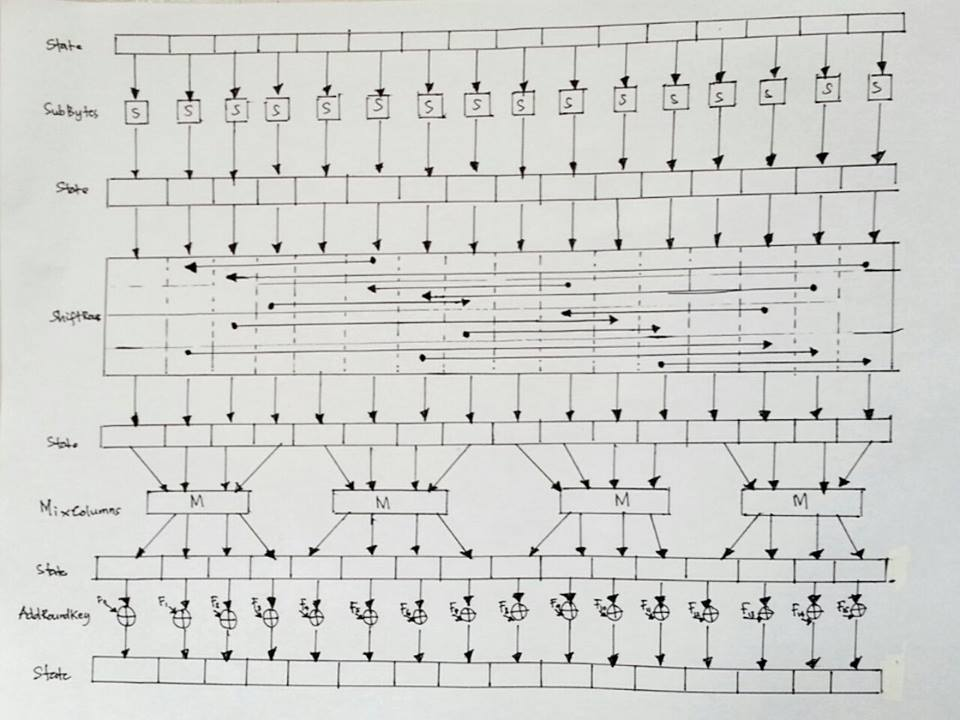
\includegraphics[scale=.6]{AESEncryptionRound2.jpg}
\caption{AES Encryption Round}
\label{AESEncryptionRound}
\end{center}
\end{figure}

\begin{figure}[h]
\begin{center}
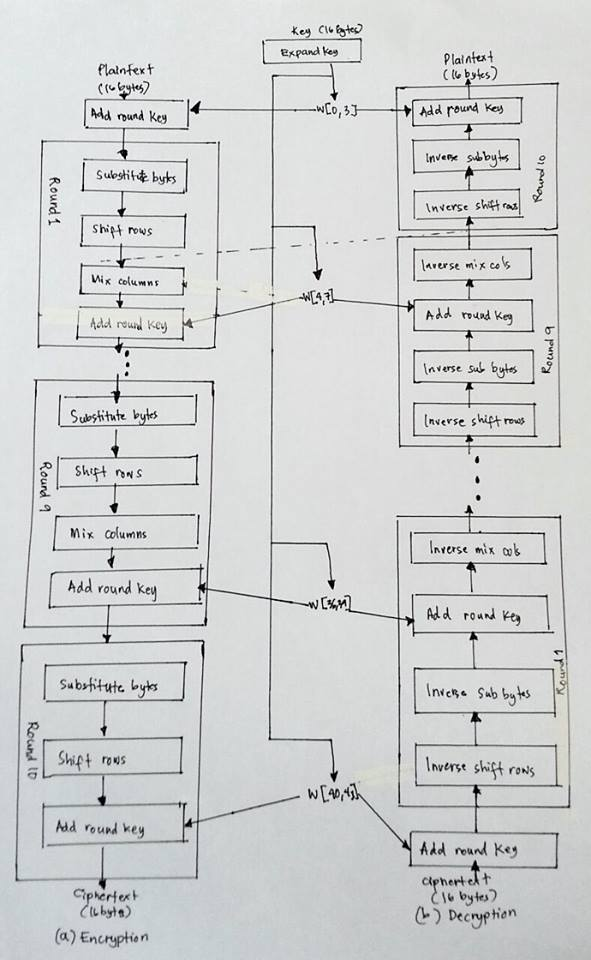
\includegraphics[scale=.6]{AESEncryptionAndDecryption2.jpg}
\caption{AES Encryption and Decryption}
\label{AESEncryptionAndDecryption}
\end{center}
\end{figure}

\paragraph{AES Decryption}
The decryption algorithm uses the expanded key in reverse order but is not identical to the encryption algorithm. \cite{stallings2011}

\paragraph{AES vs Known Attacks}
As discussed by Daemen and Rijmen\cite{daemen1999}, here are some of the known attacks during the writing of the Rijndael Block Cipher Proposal.

\subparagraph{Symmetry properties and weak keys of the DES type}
The cipher and its inverse have different components, eliminating the the possibility of weak or semi-weak keys of DES type. Equivalent keys are prevented by the non-linearity of the key expansion.

\subparagraph{Differential Cryptanalysis}
Differential Cryptanalysis Attacks are possible if the prop ratio is significantly larger than $2^{1-n}$ where n is the block length. AES has no 4-round differential trails with a prop ratio above $2^{-150}$.

\subparagraph{Linear Cryptanalysis}
Linear Cryptanalysis Attacks are possible if there are linear trails with correlation coefficients greater than $2^{n/2}$. AES has no 4-round linear trails with correlation greater than $2^{-75}$.

\subparagraph{Truncated Differentials}
Truncated Differentials are possible when the number of differential trails for certain sets of input difference patterns and output difference patterns is very large. Since AES meets the condition for truncated differentials to occur, all transformations operating on bytes were investigated. For six or more rounds, no attacks faster than exhaustive key search were found.

\subparagraph{The Square Attack}
The Square attack is an attack dedicated to the Square. It takes advantage of the byte-oriented structure of Square Ciphers. AES inherits many properties form Square cipher therefor AES is also vulnerable to this type of attack.

The Square attack is found to be faster than exhaustive key search but experiments also showed that there were no extensions to 7 rounds faster than exhaustive key search.

\subparagraph{Interpolation Attacks}
Interpolation attacks are feasible if the cipher components have a compact algebraic expression and can be mixed to provide expressions with manageable complexity. AES prevents these attacks (for more than a few rounds) through its complicated expression of the S-box in GF($2^{8}$) together with the effect of diffusion layer.

\subparagraph{Weak Keys as in IDEA}
These weak keys typically occur in ciphers with non-linear operations depending on the actual key value. In AES, weak keys are prevented by applying the keys using EXOR and putting all non-linearity in the S-box.

\subparagraph{Related-key attacks}
Related-key attacks can be achieved through using different keys with a chosen relation in different cipher operations. This attack is prevented by AES through its high diffusion and non-linearity.

\paragraph{Limitations of AES}
As discussed by Daemen and Rijmen\cite{daemen1999}, here are some of the known limitations of the AES.
\begin{itemize}
\item Since the inverse cipher takes moire code and cycles, the inverse cipher is less likely to be implemented on a smart card than the cipher itself.
\item The cipher and its inverse has different codes and/or tables.
\item The inverse cipher cannot fully re-use the circuitry implementing the cipher.
\end{itemize}

\subsubsection{Stream Ciphers}
Stream ciphers typically encrypts plaintext one byte at a time, although may differ depending on the design. In the structure of the stream ciphers, a key is input to a pseudo-random bit generator that produces a stream of 8-bit random numbers. This stream of random numbers is called a \textbf{keystream} which is combined one byte at a time with the plaintext using the bit-wise exclusive-OR (XOR) operation \cite{stallings2011}. For example:
\\

encrypt
\begin{tabular}{r l}
11001100 & plaintext\\
$\oplus$ 01101100 & key stream\\
\hline
10100000 & ciphertext
\end{tabular}
\\
\\

decrypt
\begin{tabular}{r l}
10100000 & ciphertext\\
$\oplus$ 01101100 & key stream\\
\hline
11001100 & plaintext
\end{tabular}
\\

A stream cipher can be as secure as a block cipher of comparable length if used with a properly designed pseudo-random number generator.

\subsubsection{RC4}
RC4 is a stream cipher designed by Ron Rivest of RSA Security in 1987. It is used in the Secure Sockets Layer/Transport Layer Security (SSL/TLS) standards that have been defined for communication between Web browsers and servers. It is also used in the Wired Equivalent Privacy (WEP) protocol and WiFi Protected Access (WPA) protocol that are part of the IEEE 802.11 wireless LAN standard \cite{stallings2011}.

A variable-length key of from 1 to 256 bytes is used to initialize a 256-byte state table \cite{mousa2006}. The state table is used for subsequent generation of pseudo-random bits and then to generate a pseudo-random stream which is XORed with the plaintext to give the ciphertext.

The algorithm can be broken into two stages: initialization and operation. In the initialization stage, the state table \textbf{S} is populated using \textbf{K} as a seed. Once the state table is initialized, it continues to be modified in a systematic pattern as data is encrypted. The initialization process is summarized in the pseudocode below:

\begin{algorithmic}
\State $j = 0$
\For{$i = 0 \to 255$}
	\State $S[i] = i$
\EndFor
\State $j = 0$
\For{$i = 0 \to 255$}
	\State $j = (j + S[i] + K[i]) mod 256$
	\State $swap(S[i], S[j])$
\EndFor
\end{algorithmic}

Stream generation involves cycling through all the elements of the state table, and for each S[i], swapping S[i] with another byte in \textbf{S} according to a scheme dictated by the current configuration of \textbf{S}. After S[255], the process continues starting over again at S[0].

\begin{algorithmic}
\State $i, j = 0$
\While{$true$}
	\State $i = (i + 1) mod 256$
	\State $j = (j + S[i]) mod 256$
	\State $swap(S[i], S[j])$
	\State $t = (S[i] + S[j]) mod 256$
	\State $k = S[t]$
\EndWhile
\end{algorithmic}

To encrypt, XOR the value \textit{k} with the next byte of plaintext. To decrypt, XOR the value \textit{k} with the next byte of ciphertext.

According to Mousa and Hamad \cite{mousa2006}, the speed of encryption or decryption time for RC4 is directly related to the encryption key length and to the data file size.

\section{Asymmetric Ciphers}

Cryptographic systems rely on keys for encryption and decryption.
Traditionally, a single key is required to encrypt and to decrypt.
In order for the recipient of the encrypted message to be decrypted
by the recipient, the key must also be transmitted. However, sending
the key over the channel (normal channel) where the actual message
will be sent is insecure. The key must be transmitted on a different
and secure channel (key channel)\cite{merkle_secure_1978}. This secure
channel where the key should be transmitted cannot be used for normal
transmission because it is costly and sometimes difficult for users
to access and use\cite{merkle_secure_1978}. This begs the question
whether it is possible to send encrypted messages in such a way that
the key can also be transmitted over the normal (insecure) channel
and still achieve secure communication. In this section, we focus
on solving this problem by describing the relevant and important work
on asymmetric ciphers. Figure 5 describes the flow in asymmetric cryptography.

\begin{figure}[h]
\caption{Flow of messages from source to destination.}
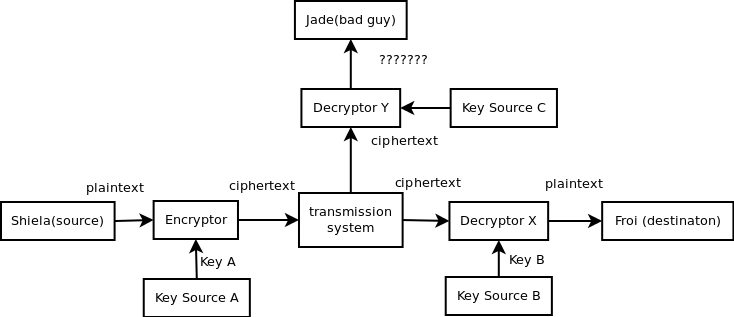
\includegraphics[scale=0.45]{flowchart1}
\end{figure}



\subsection{Merkle (1978)}

Secure communication, as described by Merkle\cite{merkle_secure_1978},
allows two parties to communicate in a private manner even though
a third party tries its best to learn what is being communicated.
We refer to the two parties as Froi and Shiela, and the third party
as Jade (Figure 5). Since the key channel is important, the following
describes the characteristics of the channel in relation to Jade.
\begin{enumerate}
\item All attempts by Jade to change the messages on the key channel are
detectable.
\item Jade will not be able to know the actual content of any message passing
on the key channel.
\end{enumerate}
The approach by Merkle relaxes the second condition: It is not necessary
for Jade not to know what is being sent in the key channel, he can
even know everything passing on it. The challenge then is how to securely
distribute the key satisfying the conditions above. If Froi and Shiela
have agreed upon a key, and the work needed by Jade to find the key
is much higher than the effort by Froi and Shiela needed to generate
the key , then it is a solution. The effort by Jade should be exponentially
higher compared to the effort by Froi or Shiela for a method to be
considered a solution. 

Merkle's method uses the concept of puzzles\cite{merkle_secure_1978}.
A puzzle is a cryptogram that is meant to be solved. Any encryption
function can be used to generate a puzzle. To allow the puzzle to
be solved, the key size (N) used in the encryption function is restricted.
The difficulty of solving a puzzle can be controlled by adjusting
the size of N. A very large size (in bits) of N will make it very
difficult to solve the puzzle. In addition, in order to be able to
solve the puzzle, some redundancy is needed. Redundancy is introduced
by encrypting, along with the original message, some constant known
to Froi, Shiela, and Jade. The absence of the constant when a puzzle
is decrypted would mean that a wrong key has been used. 

Let us consider the scenario when Shiela wishes to send a message
to Froi. First, they both agree on the value of N to use. Shiela then
generates N puzzles and transmits these N puzzles to Froi using the
key channel. Each puzzle generated will have a puzzle ID and puzzle
key. The puzzle ID uniquely identifies each puzzle. The puzzle key
on the other hand will be used in future communications that will
happen once this puzzle has been solved. 

When Froi receives the N puzzles, he selects a puzzle at random and
attempts to solve the puzzle, with the amount of effort required,
as defined by the size of the key space specified by Shiela. After
solving a puzzle, Froi sends the puzzle ID back to Shiela using the
key channel. The puzzle key, associated with the puzzle ID sent by
Froi, is then used for future communications, this time over the normal
channel. At this point Jade knows the puzzle ID, since it was sent
using the key channel, but not the puzzle key. If Jade wants to know
the key, then he must solve puzzles randomly and check the puzzle
ID if it matches the one sent by Froi back to Shiela. This will take
Jade a long time to solve. To put it formally, Jade will require $O(N^{2})$
effort to determine the key whereas Froi will only need, on the average,
$O(N)$. The function below generates the puzzles sent by Shiela to
Froi. The encryption function is arbitrary.

\begin{lstlisting}[language=C,numbers=left]
void generate_puzzle()
{
   bit_string id, key, c, random_key, puzzle, k1, k2;
   int i;

   k1 = rand(MAXINT);
   k2 = rand(MAXINT);
   c = rand(MAXINT);
   send(c);
   for (i=0; i<N; i++)
   {
      id = encryption_function(k1,i);
      key = encryption_function(k2, i);
      random_key = rand(c*N);
      puzzle = encryption_function(random_key,id,key,c);
      send(puzzle);
   }
}
\end{lstlisting}


The code below is executed on Froi's side.

\begin{lstlisting}[language=C,numbers=left]
void get_id()
{
   bit_string id, key, c, selected_puzzle_id, the_puzzle, current_puzzle,
              temp_constant;
   int i;
   
   selected_puzzle_id = rand(N);
   receive(c);
   for (i=0; i<N; i++)
   {
      receive(currrent_puzzle);
      if (i == selected_puzzle_id)
         the_puzzle = current_puzzle;
   }
   for (i=0;i<(c*N);i++)
   {
      id = get_id(finverse(i, the_puzzle));  
      key = get_key(finverse(i, the_puzzle));
      temp_constant = get_constant(finverse(i, the_puzzle));
      if (temp_constant == c)
         send(id);
   }
}
\end{lstlisting}


Once Shiela receives the the puzzle ID from Froi, then the following
code will be executed. key will be used for subsequent communications
between the two.

\begin{lstlisting}[language=C,numbers=left]
void continue_transmission()
{
   receive(ID);
   key = encryption_function(k2, ID);
}
\end{lstlisting}


The approach by Merkle requires an effort of $O(N^{2})$ from Jade
to get the key. However, in todays available computing resources,
this can be easily broken. The possibility of exponential methods
will be more attractive. Also the amount of information sent during
the initial setup of the communication is large because N puzzles,
consequently N keys, are sent initially.


\subsection{Diffie-Helman (1976)}

The work by Diffie and Helman\cite{diffie_new_1976} proposed a method
such that only one ``key'' needs to be exchanged and in addition
the time required from Jade to perform cryptanalysis is exponential.
In addition, it allows authentication because its use allows it to
be tied to a public file of user information. Shiela can authenticate
Froi and vice versa. 

Diffie and Helman differentiate \textit{public key cryptosystems}
and \textit{public key distribution systems}. We let ${K}$ be the
finite key space from which keys $K$ can be obtained and ${M}$ be
the finite message space where messages $M$ are derived. A \textit{public
key cryptosystem} is a pair of families of algorithms ${E_{k}}$ and${D_{k}}$
which represent invertible transformations\cite{diffie_new_1976}.
\[
E_{k}:\{M\}\rightarrow\{M\}
\]


\[
D_{k}:\{M\}\rightarrow\{M\}
\]


such that 
\begin{enumerate}
\item for every key $K$, $E_{k}$ is the inverse of $D_{k}$,
\item for every $K$ and $M$, the algorithms $E_{k}$ and $D_{k}$ are
easy to compute,
\item for almost every $K$, each easily computed algorithm equivalent to
$D_{k}$ is computationally infeasible to derive from $E_{k}$,
\item for every $K$, it is feasible to compute inverse pairs $E_{k}$ and
$D_{k}$ from $K$.
\end{enumerate}
Property 3 allows $E_{k}$ to be made public without compromising
$D_{k}$. Key distribution in this system is simplified. Users generate
two keys, an enciphering key $E$ and a deciphering key $D$. $E$
can be made public but $D$ is kept privately by the user. Any entity
who would like to send messages to a user can use the publicly available
$E$ to encrypt messages but only the user can decrypt the message
using $D$. In their paper, Diffie and Helman gave an example public
key cryptosystem by multiplying a binary n-vector message m with an
invertible binary n x n matrix E. However, this approach is not practical.

Merkle's\cite{merkle_secure_1978} work was classified by Diffie and
Helman as \textit{public key distribution system} and highlighted
its limitations specifically its high transmission overhead again
because of sending N puzzles initially. The proposed system is similar
to the public key cryptosystem described above, but unlike Merkle's
technique, Diffie and Helman approach allows the authentication of
users by making the public file read-only\cite{diffie_new_1976}. 

The technique proposed is dependent on the difficulty of computing
$logs\: mod\: q$ where q is a prime number representing the number
of elements of a finite field. Users generate independent random numbers
$X_{i}$ from the set of integers $\left\{ 1,2,...,q-1\right\} $.
The users keep these numbers but the computed value 
\[
Y_{i}=\alpha^{X_{i}}mod\: q
\]


is placed publicly together with the user information( such as name
and email). 

Consider for example Shiela and Froi would like to talk to each other
privately. They are going to use the key $K_{Shiela,Froi}$below after
they generate $X_{Shiela}$and $X_{Froi}$ and published $Y_{Shiela}$
and $Y_{Froi}$.

\[
K_{Shiela,Froi}=\alpha^{X_{Shiela}X_{Froi}}mod\: q
\]


Shiela will be able to obtain $K_{Shiela,Froi}$ by using the public
file $Y_{Froi}$ and then computing
\[
K_{Shiela,Froi}=Y_{Froi}^{X_{Shiela}}mod\: q
\]
 
\[
=(\alpha^{X_{Froi}})^{X_{Shiela}}mod\: q
\]


\[
=\alpha^{X_{Froi}X_{Shiela}}=\alpha^{X_{Shiela}X_{Froi}}mod\: q
\]


Froi will be able to obtain the key in the same manner. 
\[
K_{Sheila,Froi}=Y_{Shiela}^{X_{Froi}}mod\: q
\]
 

Jade might be able to compute$K_{Shiela,Froi}$ from $Y_{Shiela}$
and $Y_{Froi}$ by computing

\[
K_{Shiela,Froi}=Y_{Shiela}^{(\log_{\alpha}Y_{Froi})}mod\: q
\]


However, if Jade is to perform this computation, it will take him
a long time to do so. This system takes advantage of the fact that
$logs\: mod\: q$ are expensive to compute.


\subsection{Rivest-Shamir-Adleman (1978)}

The RSA algorithm by Rivest, Shamir, and Andleman was inspired by
the work of Diffie and Helman. Despite the breakthrough in Diffie
and Helman's work in public key cryptosystems, they did not present
any practical implementation that can be used in actual systems. The
creators of RSA took the work further by presenting a practical and
efficient implementation. Given an encryption procedure \textbf{E}
,a decryption procedure \textbf{D}, and a message \textbf{P}, a public
key cryptosystem has the following properties\cite{rivest_method_1978}:
\begin{enumerate}
\item Decrypting an encrypted \textbf{P} results to \textbf{P}. \textbf{D}(\textbf{E}(\textbf{P}))
= \textbf{P.}
\item \textbf{D} and \textbf{E} are easy to compute.
\item Publicly revealing \textbf{E} does not mean that it will be easy to
compute \textbf{D} from \textbf{E}. It should be difficult or inefficient
to compute \textbf{D} from \textbf{E}.
\item If \textbf{P} is decrypted and then encrypted, \textbf{P} is the result.
\textbf{E}(\textbf{D}(\textbf{P})) = \textbf{P}.
\end{enumerate}
The encryption and decryption functions rely on a key such that the
security of the functions or procedures rests on the security of the
key. If \textbf{E} satisfies properties 1-3 is referred to as ``trap-door
one way function''. If it also satisfies property 4 then it is referred
to as ``trap-door one-way permutation''. In public key cryptosystems
the usual ``setup'' time is simply the time it takes to make the
encryption function public.%
\footnote{In their paper, it is the encryption function that is made public.
Other researchers talk about keys being made public, not the functions.
Essentially, however, there is a one-to-one correspondence between
the encryption function and the key.%
} If Shiela wants to encrypt a message \textbf{P}, for Froi, with the
key \textbf{(e, n)}, she must first represent \textbf{P} as an integer
between \textbf{0} and \textbf{n-1}, where \textbf{e} and \textbf{n}
are positive integers. \textbf{P} is then encrypted to generate the
ciphertext \textbf{C} by raising \textbf{P} to the $e^{th}$ power
modulo \textbf{n}. The decryption process will raise the ciphertext
to another power \textbf{d} modulo \textbf{n}. The mathematical formulation
is shown below. 
\[
C\equiv E(P)\equiv P^{e}(mod\: n)
\]


\[
P\equiv D(C)\equiv C^{d}(mod\: n)
\]


The the length of the original message is not increased during the
encryption process. The pairs \textbf{(e,n)} and \textbf{(d,n)} are
the encryption keys and decryption keys respectively. The encryption
key is made public and the decryption key is private to the user.
In the above example, \textbf{(e,n)} is the public key of Froi, he
can decrypt the message using \textbf{(d,n)} which is in his possession.
The security of the approach is based on the security of the keys,
thus the keys must be selected well. \textbf{n} is computed as a product
of two large random primes \textbf{p} and \textbf{q}, \textbf{n =
p {*} q}. Although \textbf{n} will be made public, \textbf{p} and
\textbf{q} will not, which hides the way \textbf{d} can be derived
from \textbf{e}. \textbf{d} is a random integer such that $gcd(d,(p-1)*(q-1))=1$.
\textbf{e} is computed from \textbf{p}, \textbf{q}, and \textbf{d}
such that

\[
e*d\equiv1(mod(p-1)*(q-1))
\]


This requirement guarantees that properties 1 and 4 above are satisfied,
which means that \textbf{E} and \textbf{D} are inverse permutations.
Although Diffie and Helman\cite{diffie_new_1976} also used exponentiation
and modulo in determining a common key to be used, their approach
is not based on a ``trap-door one-way permutation'' which means
that property 4 is satisfied.

The creators of RSA presented an efficient implementation of the of
their approach. Note that the basic operations in the encryption and
decryption process are exponentiation and division (to compute the
remainder). The technique is called ``exponentiation by repeated
squaring and multiplication.'' The technique presented will need
at most $2*\log_{2}(e)$ multiplications and $2*\log_{2}(e)$ divisions.
The encryption and decryption algorithms are shown below.
\begin{lstlisting}[language=C,numbers=left]
long E(long P,int e, int n)
{
   long C=1;
   int i;
   
   for (i=k;k==0;k--)
   {
      C = (C * C) % n;
      if (bit(i,e) == 1) /* bit(i,e) returns the ith bit of e*/
         C = (C * P) % n;
   }
   return C;  
}

long D(long C,int d, int n)
{
   long P=1;
   int i;
   
   for (i=k;k==0;k--)
   {
      P = (P * P) % n;
      if (bit(i,d) == 1) /* bit(i,d) returns the ith bit of d*/
         P = (P * C) % n;
   }
   return P;  
}
\end{lstlisting}


It can be seen that the RSA encryption and decryption algorithms are
straightforward to implement. The challenge however is in the selection
of the keys which is dependent of several parameters (e, d, n). In
their paper, the creators of RSA also presented several approaches
how to generate these parameters to guarantee the security.

\bibliographystyle{unsrt}
\bibliography{references}
\nocite{*}

\end{document}
